\chapter{LMDPs}

\begin{figure}
\centering
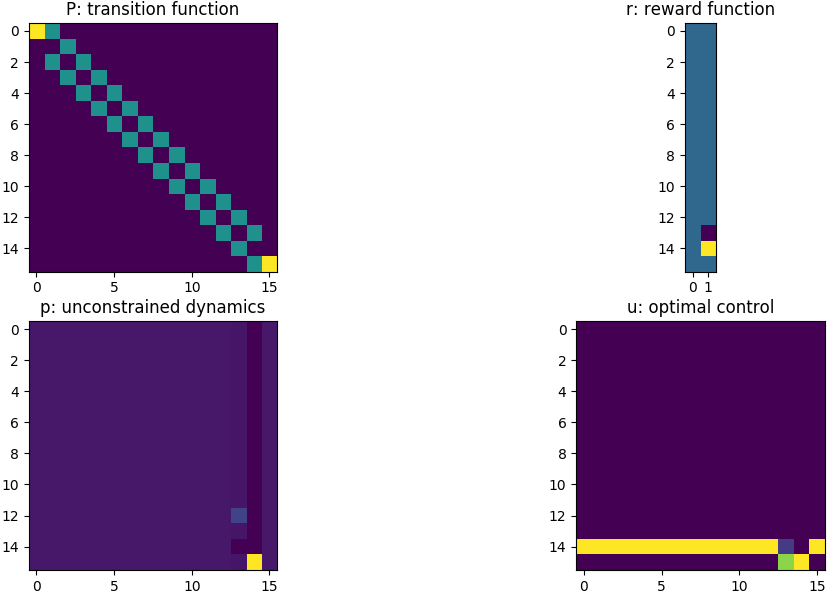
\includegraphics[width=0.75\textwidth,height=0.5\textheight]{../../pictures/figures/chain-test-zero-rewards.png}
\caption{'A chain problem with zero reward on all states except the last two.'}
\end{figure}

\begin{figure}
\centering
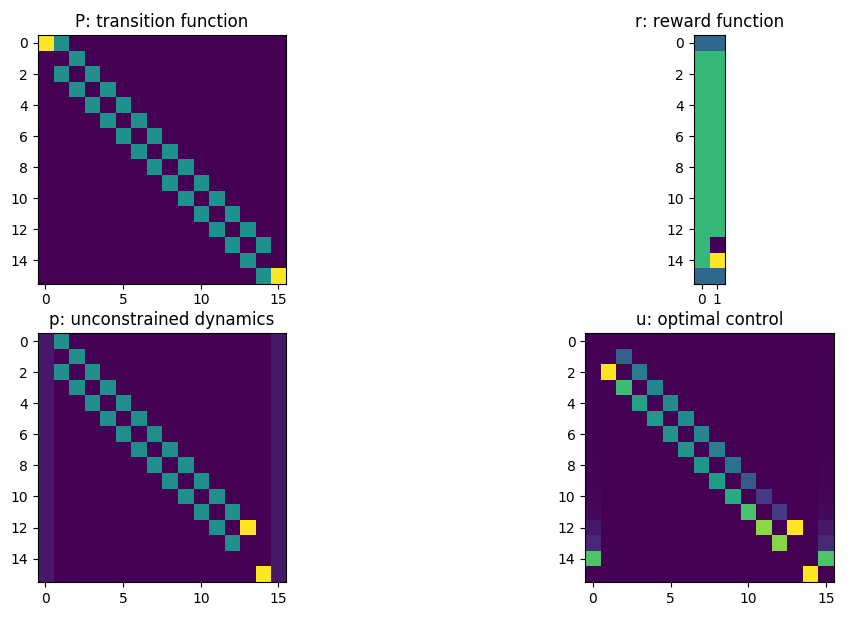
\includegraphics[width=0.75\textwidth,height=0.5\textheight]{../../pictures/figures/chain-test-pos-rewards.png}
\caption{'A chain problem with positive rewards applied to all states.'}
\end{figure}

\begin{figure}
\centering
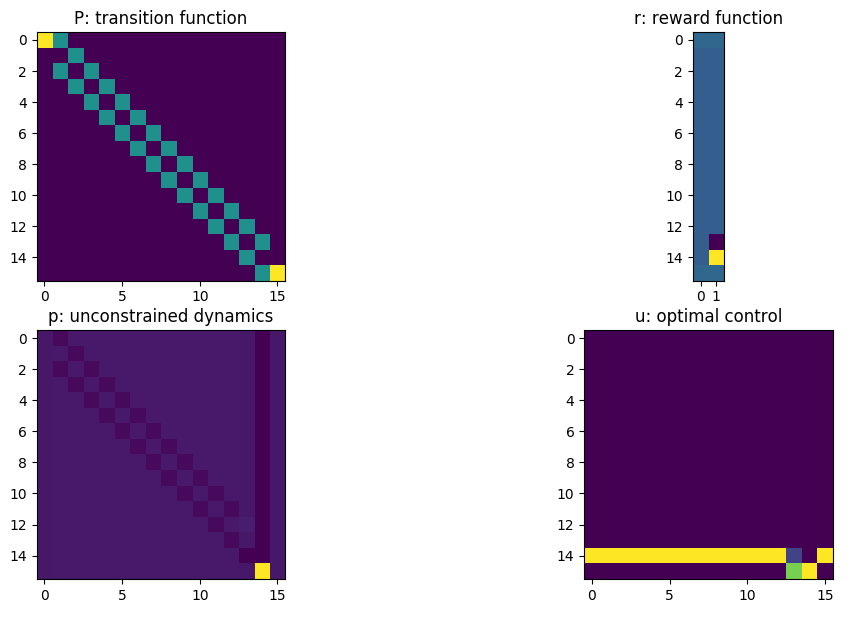
\includegraphics[width=0.75\textwidth,height=0.5\textheight]{../../pictures/figures/chain-test-neg-rewards.png}
\caption{'A chain problem with negative rewards applied to all states'}
\end{figure}


In the original Todorov paper, they derive the LMDP equations for
minimising a cost function. This maximisation derivation just changes a
few negative signs around. Although there is also a change in the
interpretation of what the unconstrained dynamics are doing. \ldots{}?
